\documentclass{article}
\usepackage[spanish]{babel}
\usepackage{graphicx}
\usepackage[utf8]{inputenc}
\usepackage[spanish]{babel}
\usepackage{natbib}
\usepackage{float}
\usepackage{amsmath}
\usepackage{amssymb}

\usepackage{tikz}
\usetikzlibrary{shapes.geometric, arrows}

\tikzstyle{startstop} = [rectangle, rounded corners, minimum width=3cm, minimum height=1cm,text centered, draw=black, fill=red!30]
\tikzstyle{process} = [rectangle, minimum width=3cm, minimum height=1cm, text centered, draw=black, fill=orange!30]
\tikzstyle{decision} = [diamond, minimum width=1.5cm, minimum height=0.8cm, text centered, draw=black, fill=green!30,font=\footnotesize]
\tikzstyle{arrow} = [thick,->,>=stealth]

\title{Agosto}
\author{José Adrián Rodríguez González}
\date{Septiembre 2024}
\begin{document}
\maketitle
\section{Introducción}
Para este mes se estudiara los algoritmos genéticos, sus principios, su flujo de trabajo, a su vez como ejemplos prácticos para entender los conceptos teóricos.
\subsection{¿Qué es un algoritmo génetico?}
Es un algoritmo que procede del principio básico de la evolución\citep{10.7551/mitpress/1090.001.0001}, en el que las como las especies se adaptan a su entorno. Esta visión fue desarrollada en los años 70's e implementada en lenguajes como C, o C++. Es una metodoogía muy útil ante problemas complejos en los que no hay una solución directa, o problemas en los que la incertidubre puede entrar en juego. Además, los algoritmos genéticos pueden ser de utilidad en la elección o toma de decisiones en algun modelo de aprendizaje automatico. Muchas veces se utilizan algoritmos genéticos binarios para procesar los problemas.
El algoritmo se define por el siguiente diagrama de flujo,\citep{10.5555/559152}
\begin{figure}[H]
\begin{tikzpicture}[node distance=2cm]

    \node (start) [startstop] {Inicio};
    \node (init) [process, below of=start] {Inicialización de la población};
    \node (fitness) [process, below of=init] {Evaluación de aptitud};
    \node(eval)[process, right of=fitness, xshift=2.5cm]{Asignación de fitness};
    \node(cond)[decision, below of=fitness, yshift=-1.25cm,xshift=1.3cm]{¿Criterio de parada?};
    \node(Reproduction)[process, right of=cond, xshift=2.25cm]{Selección};
    \node(Crossover)[process, below of=Reproduction]{Cruce};
    \node(mutation)[process, left of=Crossover,xshift=-8cm]{Mutación};
    \node(gen)[process, above of=mutation,yshift=3.2cm]{gen=gen+1};
    \node (end) [startstop,left of=cond,xshift=-2cm] {Pare};

    \draw [arrow] (start) -- (init);
    \draw [arrow] (init) -- (fitness);
    \draw [arrow] (fitness) -- (eval);
    \draw [arrow] (eval) -- (cond);
    \draw [arrow] (cond) -- node[anchor=east,yshift=0.5 cm] {No} (Reproduction);
    \draw [arrow] (cond) -- node[anchor=west,yshift=0.5 cm] {Si} (end);
    \draw [arrow] (Reproduction) -- (Crossover);
    \draw [arrow] (Crossover) -- (mutation);
    \draw [arrow] (mutation) -- (gen);
    \draw [arrow] (gen) -- (fitness);
    \label{fig:diagrama}
\end{tikzpicture}
\caption{Diagrama de flujo}
\end{figure}
    \section{Fases de un algoritmo genético.}
    \begin{itemize}
        \item Inicialización de la población: Es el proceso en el que se propone una gama de posibles soluciones a la problemática
        \item Evaluación de la aptitud: Es el proceso en el que se evaluan las posibles respuestas a nuestra problemática.
        \item Asignación de fitness: es una ponderación que se asigna ya sea por una función de restricción o por la función objetivo.
        \item Criterio de parada: El criterio es la sección en la que determina cuando parar el bucle. Este criterio puede darse cuando se encuentre el resultado esperado para la función objetivo o por alguna función de restricción.
        \item Selección: Se seleccionan los resultados que mejor resultados obtuvieron, sin embargo, también se puede realizar este proceso por metódo de combate, de tal forma que se evita el seleccionar posibles padres que tengan muchas caracterísitcas en común
        \item Cruce: Se reproducen los padres seleccionados y se obtienen hijos o nuevos posibles resultados
        \item Mutación: En este proceso, se le da un pequeño porcentaje como factor, de tal forma que le ayudará a ser ligeramente distinto a sus padres.
        \item $gen=gen+1$: este proceso se hará en la siguiente generación de hijos.
    \end{itemize}
    Los algoritmos evolutivos pueden ser reproducidos n cantidad de generaciones, por lo tanto es necesario una condición que permita detener el proceso.\citep{kubat2021introduction}
    \section{Casos prácticos.}
    Para poder comprender el funcionamiento y el como opera un algoritmo génetico, se analizaron códigos desarrollados en python. \footnote{Código proporcionado por José Salvador González}
    El problema a resolver era el del viajero, ¿cual es la ruta más corta para ir a n ciudades sin recorrer el mismo camino ni la misma ciudad.
\begin{figure}[H]
    \centering
    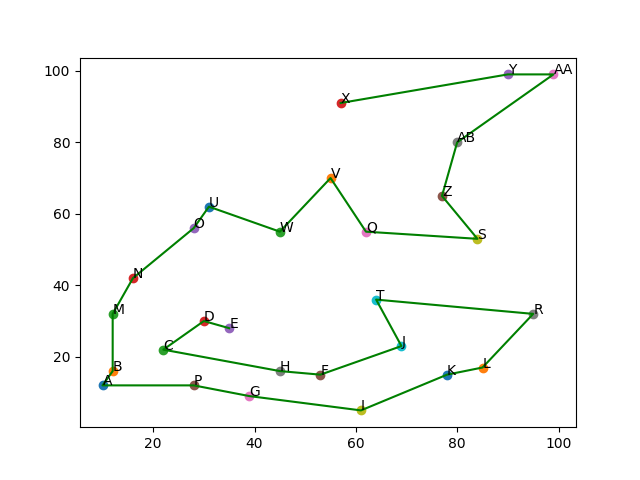
\includegraphics[width=0.5\textwidth]{Figure_2.png} % Cambia 'nombre_de_la_imagen' por el nombre real del archivo de la imagen
    \caption{El problema del viajero}
    \label{fig:miimagen}
\end{figure}
Del cuál, arrojo el siguiente resultado con 350 generaciones.

BEST PATH : ['E' 'D' 'C' 'H' 'F' 'J' 'T' 'R' 'L' 'K' 'I' 'G' 'P' 'A' 'B' 'M' 'N' 'O'
 'U' 'W' 'V' 'Q' 'S' 'Z' 'AB' 'AA' 'Y' 'X']

FITNESS : 436.12724616750086

En este proceso, se pudieron analizar los pasos de algoritmos genéticos. Además, también se pudo desarrollar una segunda práctica para maximizar una función
Siendo $$f(x)=x-x^2 $$
Se puede encontrar su máximo por su primera derivada, siendo 

$$x=0.5, f(x)=0.25$$
En este caso, se aplica el proceso descrito por \ref{fig:diagrama} y se itero 100 veces, de tal forma que el algoritmo encontró $ x=0.50 ,f (x)=0.25$.
Conociendo el principio básico del algoritmo genético a su vez que de la naturaleza del problema, pueden ser una herramienta poderosa en problemas demasiado complejos. Estos algoritmos son apliamente utilziados en combinación con los principios de la lógica difusa.
\bibliographystyle{apalike}
\bibliography{reference}
\end{document}